
%(BEGIN_QUESTION)
% Copyright 2010, Tony R. Kuphaldt, released under the Creative Commons Attribution License (v 1.0)
% This means you may do almost anything with this work of mine, so long as you give me proper credit

This temperature control system uses a pneumatic transmitter and controller to maintain constant temperature at the outlet of the heat exchanger:

$$\includegraphics[width=15.5cm]{i00066x01.eps}$$

A routine maintenance task you are assigned is to ``stroke-test'' the control valve to verify that its travel is not impeded or its calibration too far off.  The only problem is, this must be done while the process is ``live'' (feed flow being heated) and the pneumatic controller has no manual mode.

\vskip 10pt

Outline a plan to follow allowing you to stroke-test this control valve with minimal interruption to the process.  Points to address include:

\begin{itemize}
\item{} How to maintain feed temperature at setpoint while valve is being stroked
\vskip 5pt
\item{} How to stroke the valve from 0\% to 100\% of range with no manual mode in the controller
\end{itemize}

\vfil

\underbar{file i00066}
\eject
%(END_QUESTION)





%(BEGIN_ANSWER)

This is a graded question -- no answers or hints given!

%(END_ANSWER)





%(BEGIN_NOTES)

Somehow, we must find a way to move the control valve throughout its entire range of travel without affecting the flow of steam through the heat exchanger.  Thankfully, we have block and bypass valves installed for the purpose of isolating the control valve from the process flow.  Closing the block valves will prevent flow from going through the control valve, while opening the bypass valve will provide an alternative pathway around the control valve for the steam so that the heat exchanger can still receive an input of thermal energy to maintain temperature on setpoint (indicated by the temperature gauge TG).  Closing the block valves and opening the bypass valve is a procedure best done in incremental steps rather than all at once, to avoid subjecting the system to thermal shock (e.g. close one block valve just a bit, then open up the bypass valve).  If there happens to be a flowmeter located anywhere along the steam supply line, its indication will prove to be very helpful as we manually close the block valve(s) and open the bypass valve, letting us know if the steam flow has deviated much from its original value.  Of course, the temperature gauge will also tell us that, but its response will be much slower and therefore more difficult to control by.

\vskip 10pt

After the control valve has been completely blocked and bypassed, we may use a hand pump (or a precision regulator connected to an instrument air supply) to provide the ``stroking'' signal to the valve with the controller output tube disconnected from the valve.

%INDEX% Final Control Elements, valve: performing maintenance on live system

%(END_NOTES)


